\section{Introduction and Related Work}
\label{sec:intro}
Recent research in computer vision and pattern recognition has highlighted the capabilities of Convolutional Neural Networks (CNNs) to solve challenging tasks such as classification, segmentation and object detection, achieving state-of-the-art performances. 
This success has been attributed to the ability of CNNs to learn a hierarchical representation of raw input data, without relying on handcrafted features. 
As the inputs are processed through the network layers, the level of abstraction of the resulting features increases. 
Shallower layers grasp local information while deeper layers use filters whose receptive fields are much broader that therefore capture global information \cite{zeiler2014visualizing}. 

\begin{figure} 	
\centering 	
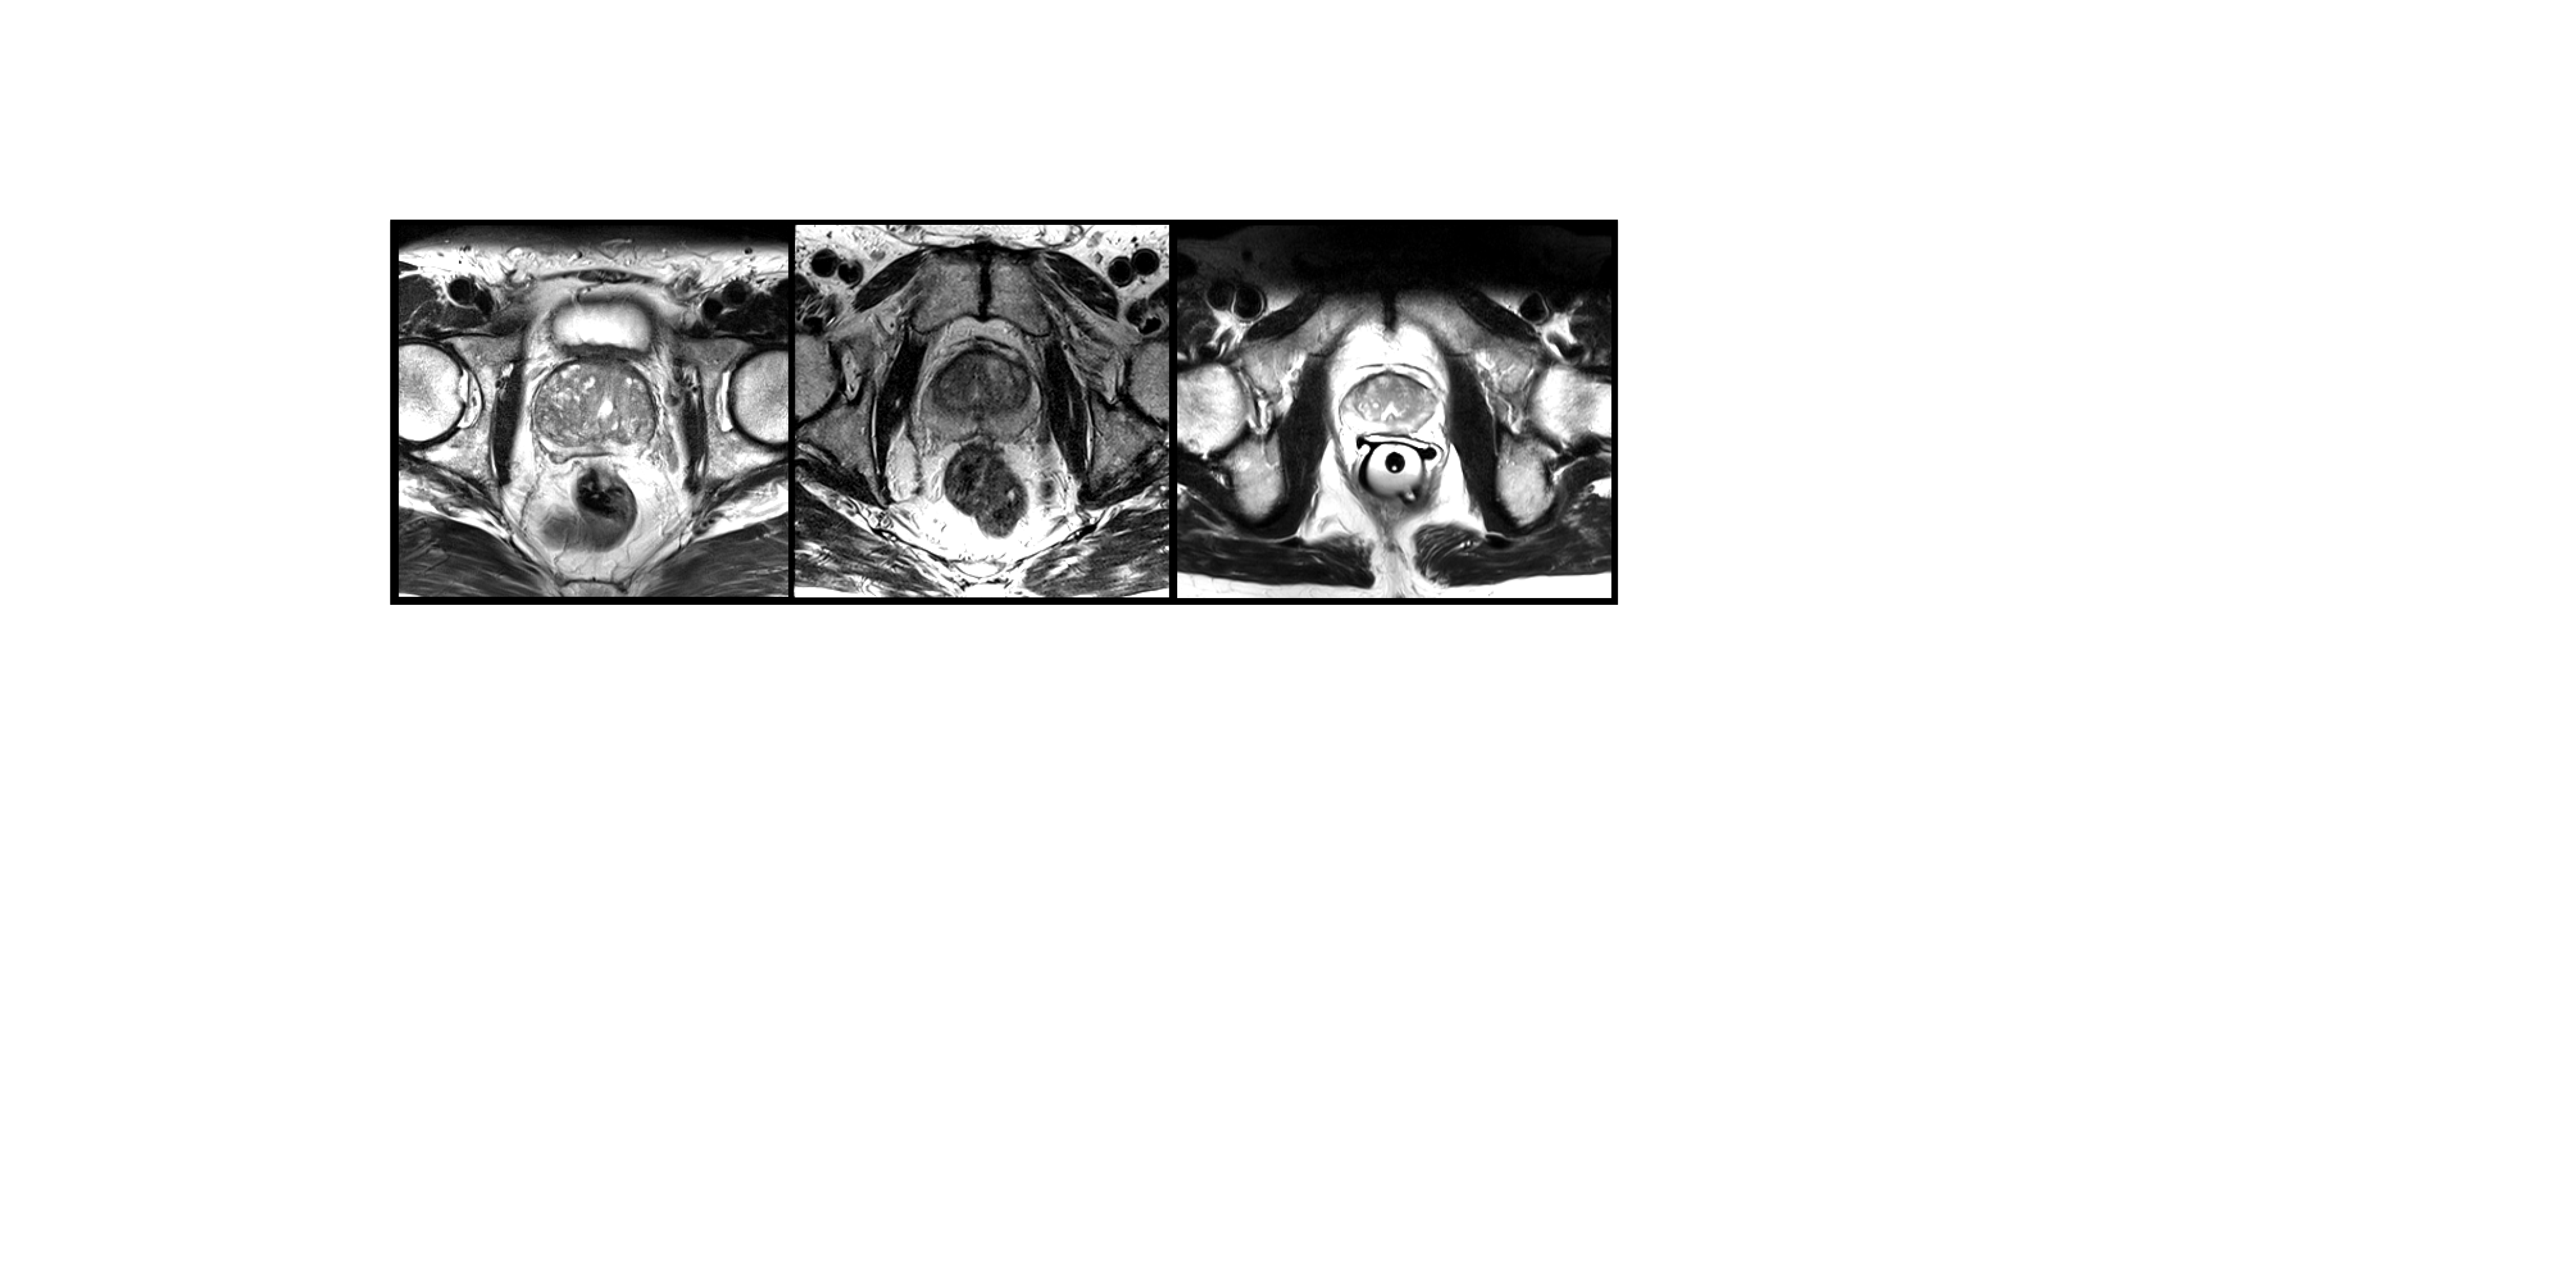
\includegraphics[scale=0.17]{anatomies.pdf} 	
\caption{Slices from MRI volumes depicting prostate. This data is part of the PROMISE2012 challenge dataset \cite{litjens2014evaluation}.} \label{fig:anatomies} 
\end{figure}

Segmentation is a highly relevant task in medical image analysis. 
Automatic delineation of organs and structures of interest is often necessary to perform tasks such as visual augmentation \cite{moradi2009augmenting}, computer assisted diagnosis \cite{porter2003combining}, interventions \cite{zettinig2015multimodal} and extraction of quantitative indices from images \cite{bernard2015standardized}. 
In particular, since diagnostic and interventional imagery often consists of 3D images, being able to perform volumetric segmentations by taking into account the whole volume content at once, has a particular relevance. 
In this work, we aim to segment prostate MRI volumes. This is a challenging task due to the wide range of appearance the prostate can assume in different scans due to deformations and variations of the intensity distribution. Moreover, MRI volumes are often affected by artefacts and distortions due to field inhomogeneity. Prostate segmentation is nevertheless an important task having clinical relevance both during diagnosis, where the volume of the prostate needs to be assessed \cite{roehrborn1999serum}, and during treatment planning, where the estimate of the anatomical boundary needs to be accurate \cite{huyskens2009qualitative,zettinig2015multimodal}. 

CNNs have been recently used for medical image segmentation. 
Early approaches obtain anatomy delineation in images or volumes by performing patch-wise image classification. Such segmentations are obtained by only considering local context and therefore are prone to failure, especially in challenging modalities such as ultrasound, where a high number of mis-classified voxel are to be expected.
Post-processing approaches such as connected components analysis normally yield no improvement and therefore, more recent works, propose to use the network predictions in combination with Markov random fields  \cite{kamnitsas2016efficient}, voting strategies \cite{milletari2016hough} or more traditional approaches such as level-sets  \cite{cha2016urinary}. 
Patch-wise approaches also suffer from efficiency issues. When densely extracted patches are processed in a CNN, a high number of computations is redundant and therefore the total algorithm runtime is high. In this case, more efficient computational schemes can be adopted.

Fully convolutional network trained end-to-end were so far applied only to 2D images both in computer vision \cite{noh2015learning,long2015fully} and microscopy image analysis \cite{ronneberger2015u}. These models, which served as an inspiration for our work, employed different network architectures and were trained to predict a segmentation mask, delineating the structures of interest, for the whole image. In \cite{noh2015learning} a pre-trained VGG network architecture \cite{simonyan2014very} was used in conjunction with its mirrored, de-convolutional, equivalent to segment RGB images by leveraging the descriptive power of the features extracted by the innermost layer. In \cite{long2015fully} three fully convolutional deep neural networks, pre-trained on a classification task, were refined to produce segmentations while in \cite{ronneberger2015u} a brand new CNN model, especially tailored to tackle biomedical image analysis problems in 2D, was proposed.

In this work we present our approach to medical image segmentation that leverages the power of a fully convolutional neural networks, trained end-to-end, to process MRI volumes. 
Differently from other recent approaches we refrain from processing the input volumes slice-wise and we propose to use volumetric convolutions instead. We propose a novel objective function based on Dice coefficient maximisation, that we optimise during training.
We demonstrate fast and accurate results on prostate MRI test volumes and we provide direct comparison with other methods which were evaluated on the same test data \footnote{Detailed results available on \url{http://promise12.grand-challenge.org/results/}}. 
%The implementation of our approach will be published upon paper acceptance.